% The paper preamble loads paper/numbers.tex and graphicx.
\subsection{An exploratory contrast: memorized wrong labels}
\label{sec:wronglabel}

The name shortcut is one rule shared across many reviews. Memorized wrong labels are a different kind of failure: many
separate associations, each tied to one training example~\cite{dankers2024memorisation}. We fine-tuned GPT-2 on 6{,}920
SST-2~\cite{socher2013sst} sentences with 15\% of the labels flipped, together with a clean twin trained on the true
labels, and measured memorization as the fraction of flipped examples that receive their wrong label
(\wlMNoisyRange{} in the noisy models).

Here the block mattered for retraining under our protocol. On corrected labels, only block~\wlPassingBlockNoisy{}
passed the mitigation criterion, removing \wlRetrainSingleNoisyRange{} of the memorization (all blocks together:
\wlRetrainAllNoisyRange). One possible explanation is that there is no shared cue for every block to learn to ignore;
each wrong label is a separate fact. The block that works is again not where the tools point: the lens places the
takeover at layer \wlTakeoverNoisyRange, the only swap that passes replaces blocks \wlSwapBlocksNoisy{} (removing \wlSwapGroupNoisyRange), and across
blocks the swap and retraining rankings show no consistent association (Spearman \wlSpearmanNoisyRange;
Fig.~\ref{fig:wronglabel-removal}). The rules of this experiment were registered, but the comparison with the name
shortcut is exploratory: it changes the dataset, task and training-set size as well as the kind of failure, so it does
not isolate the failure type.

\begin{figure}[t]
  \centering
  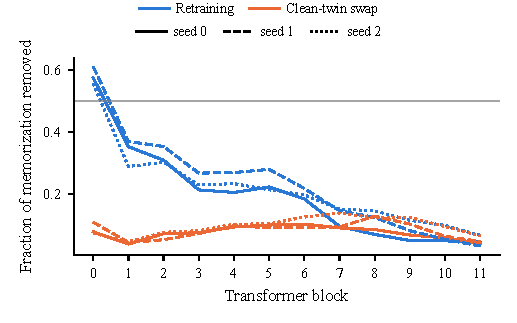
\includegraphics[width=\columnwidth]{figures/paper/fig_f_wronglabel.pdf}
  \caption{Fraction of baseline wrong-label memorization removed by
  retraining or swapping each individual block. Swaps use the
  same-seed clean twin. Line styles distinguish seeds.
  The horizontal line marks the mitigation cutoff. The full criterion
  also requires protection of accuracy.}
  \label{fig:wronglabel-removal}
\end{figure}
